\documentclass[border=10pt]{standalone}
\usepackage{tikz}
\usetikzlibrary{positioning, backgrounds}

\begin{document}

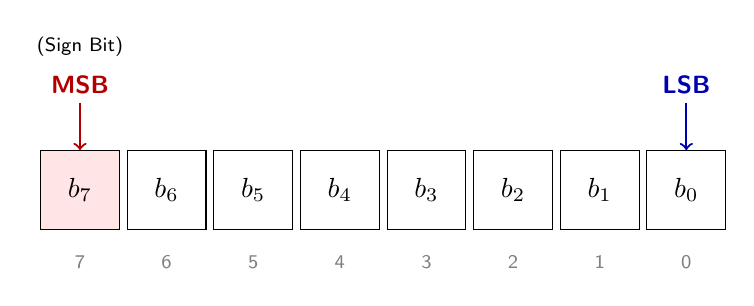
\begin{tikzpicture}[
    bitbox/.style={draw, minimum width=1cm, minimum height=1cm, align=center, font=\sffamily},
    label/.style={font=\sffamily\small, gray}
]
    % Draw bits 7 down to 0
    \foreach \i [count=\x] in {7,6,5,4,3,2,1,0} {
        % Highlight MSB (bit 7)
        \ifnum\i=7
            \node[bitbox, fill=red!10] (bit\i) at (\x*1.1, 0) {$b_{\i}$};
        \else
            \node[bitbox] (bit\i) at (\x*1.1, 0) {$b_{\i}$};
        \fi
        
        \node[below=2mm of bit\i, font=\sffamily\scriptsize, gray] {\i};
    }
    
    % MSB Indication
    \node[above=6mm of bit7, font=\bfseries\sffamily\small, text=red!70!black] (msb) {MSB};
    \draw[->, thick, red!70!black] (msb) -- (bit7.north);
    \node[above=0mm of msb, font=\sffamily\scriptsize, align=center] {(Sign Bit)};

    % LSB Indication
    \node[above=6mm of bit0, font=\bfseries\sffamily\small, text=blue!70!black] (lsb) {LSB};
    \draw[->, thick, blue!70!black] (lsb) -- (bit0.north);

\end{tikzpicture}

\end{document}
